\subsection{Aufgabenstellung und Anforderungen}
Das Ergebnis des Projekts Edubot soll ein simpel zu bedienendes, funktionales und effektives Werkzeug zum Erlernen der grundsätzlichen Arbeitsweise eines Roboters darstellen. Es soll im Anschluss an diese Diplomarbeit im Fach “Prozessregelung mit Laborübungen” verwendet werden. Das Projekt beinhaltet eine Programmierschnittstelle (API) mit der  Schüler den Roboter schnell und einfach in ihre eigenen Programme einbinden können, sowie eine Endanwendung welche zu Präsentations- und Unterrichtszwecken verwendet werden kann.
Des weiteren soll entsprechende Hardware für schulungs und präsentationszwecke zur Verfügung gestellt werden. Diese Hardware soll sowohl ein einfaches, funktionstüchtiges Robotermodell, als auch eine Softwarebasis für ein leistungsstärkeres Modell beeinhalten.
\\[0.5em]
Zusätzlich zu den erwähnten Funktionen soll ein ausführliches Dokumentations und Hilfesystem m zur Verfügung gestellt werden, um es dem Anwender zu ermöglichen, sowohl die Funktionen der API zu verstehen, als auch einen Einblick in die Funktionsweise von Anwendung und Hardware zu erlangen.
\begin{figure}[H]
  \centering
  \begin{minipage}[t]{14 cm}
  	\centering
  	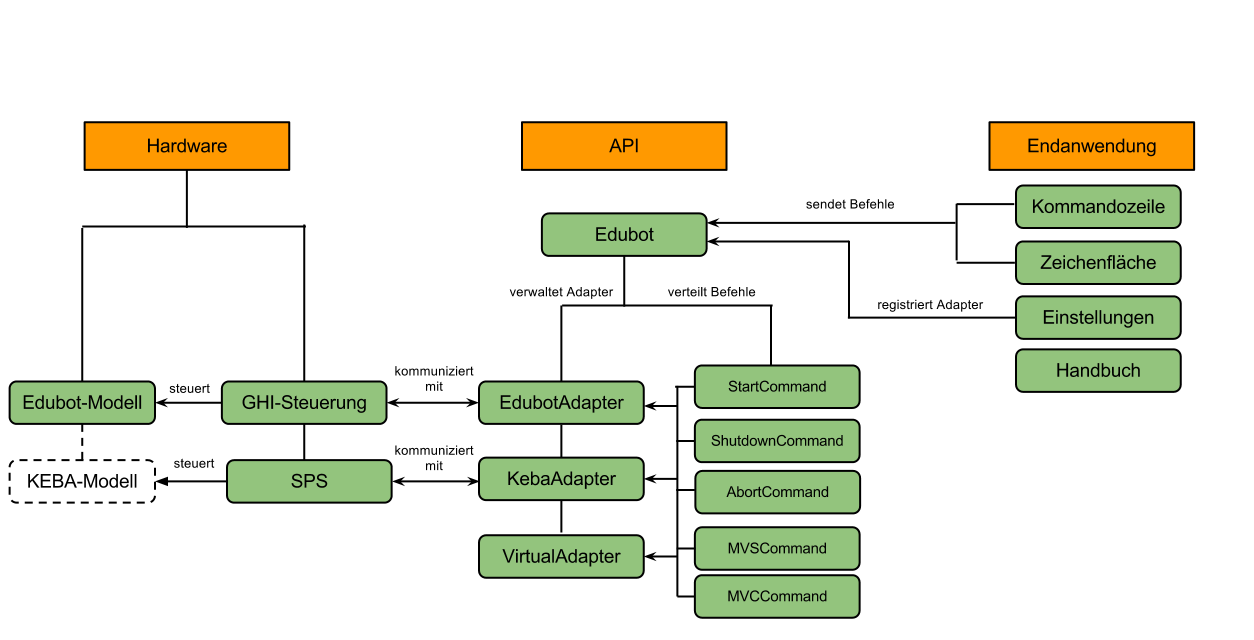
\includegraphics[width=14cm]{images/EdubotSystem} 
    \caption{Gesamtkonzept}
  \end{minipage}
\end{figure}
Dieses Kapitel dient dazu, die Anforderungen die für einen erfolgreichen Projektabschluss erforderlich sind festzulegen. Gleichzeitig stellt dieses Kapitel auch die Zieldefinition dieses Projektes dar, da es zu jeder Zeit als Hauptziel dieser Arbeit galt sämtliche in dieser Aufgabenstellung defierte und damit von unserem Auftraggeber geforderte Anforderungen zu erfüllen.

Die Folgenden Unterkapitel sollen einen detailierteren Überblick über die einzelnen Aufgaben der Teilbereiche des Projekts und die Anforderungen welche an diese gestellt werden bieten.
\subsubsection{Anwendung}
Die Edubot Endanwendung soll dem Benutzer eine Oberfläche bieten, welche ihm, über den Umweg der API, den Zugriff auf die Hardware ermöglicht. Die Anwendung soll über folgende Grundfunktionen verfügen:
\begin{itemize}
\item \textbf{Standardfunktionen und Design}\\
Um die Bedienung des Programms zu erleichtern und den Überblick über die Anwendung zu ermöglichen, soll eine einfach zu bedienende und selbsterklärende Benutzeroberfläche mit ansprechendem Desigt erstellt werden. In der Oberfläche sollen einfache Standardfunktionen eingearbeitet sein, die es beispielsweise ermöglichen in Kommandozeile oder Zeichenfläche getätigte Änderungen rückgängig zu machen und wiederherzustellen. Des weiteren soll die Möglichkeit bestehen, die in den Einstellungen vorgenommenen Änderungen zu speichern und für den nächsten Programmstart wieder aufrufbar zu machen.
\item \textbf{Einstellungen}\\
Ein Bereich zur Vornahme von Einstellungen soll alle Konfigurationsmöglichkeiten der Anwendung zusammenfassen. Dabei soll er die Möglichkeit der Auswahl, ob und auf welcher Hardware Befehle ausfgeführt werden sollen, bieten. Zusätzlich soll in den Einstellungen die Konfiguration der benötigten Verbindungsparamter möglich sein. Ebenfalls in diesem Berreich sollen sich verschiedene Konfigurationsparameter für die Visualisierung anpassen lassen. In diesem Zusammenhang sollen für die Visualisierung beispielsweise Informationen über die Länge der Achsen angegeben werden können. Wurde das physische Edubot Modell als Hardware ausgewählt, so sol automatischl eine angepasste Visualisierung mit festen Parametern angezeigt werden.
\item \textbf{Visualisierung}\\
Da die Software auch ohne das Anschließen von Hardware benutzbar sein soll, muss eine Simulation eines Roboters verfügbar sein. Es soll hier verschiedene Ansichten auf den Roboter geben. Die Visualisierung soll es ermöglichen sämtliche eingegebene Befehle unabhängig von der Hardware anhand eines 3D Modells zu Simulieren. Durch diese Funktion soll es einer größeren Anzahl von Schülern ermöglicht werden gleichzeitig mit der Software zu arbeiten und trozdem die Ergebnisse ihrer Eingaben mitzuverfolgen.
\item \textbf{Zeichenfläche}\\
Die Endanwendung soll eine einfache Zeichenfläche bieten auf welcher der Benutzer simple Standardformen und Freihandlinien zeichnen kann. Die gezeichneten Formen sollen beim drücken eines entprechenden Buttons ins einzelne Linien umgerechnet und schließlich an die API übergeben werden.
\item \textbf{Kommandozeile}\\
Ein Kommandozeilen Tool soll es ermöglichen einzelne Befehle und Befehlsketten in einer einfachen Script Sprache einzugeben. Die eingegebenen Befelle sollen über den Klick auf einen Button über die API ausgeführt werden können. Treten bei der Ausführung der Befehle Fehler auf, so sollen diese in einem entsprechenden Ausgabeberreich angezeigt werden.
Um die Eingabe in die Kommandozeile zu vereinfachen, soll diese zusätzlich passende anzeigen zu lassen und nach Auswahl anzeigen zu lassen. Diese Funktion soll der aus diversen Entwicklungsumgebungen bekannten Autocomplete Funktion ähneln.
\item \textbf{Handbuch}\\
Die Anwendersoftware soll einen eigenen Berreich für die Anzeige eines Handbuches bieten. Das zur Verfügung gestellte Handbuch soll nicht nur einen groben Überblick über die Bedienung der Anwendung geben, sondern vielmehr einen erweiterten Einblick in die Funktionsweise aller Teilberreiche diese Projekts bieten. Es soll dem Leser ermöglicht werden mehr über Robotik und den Aufbau eines einfachen Roboters zu erfahren und mitgelieferte API zu nutzen.
\end{itemize}
\subsubsection{Hardwareinterface - API}
Eine Programmierschnittstelle in Form einer als "'.dll"' einbindbaren Programmbibliothek soll alle wesentlichen Aufgaben übernehmen die zum Betrieb eines Roboters nötig sind. Eine Anwendung die einen Roboter benutzen soll nur noch die eintsprechenden Funktionenen der API aufrufen müssen. Grundsätzlich soll die API nicht an spezielle Hardware gebunden sein, sondern die Möglichkeit bieten durch entsprechende Strukturen das Einbinden von eigenen Konstruktionen ermöglichen. 
Die von der API zu übernehmenden Aufgaben sind vor allem:
\begin{itemize}
\item \textbf{Invers Kinemematik}\\
Das Hardwareinterface soll die Aufgabe der Berechnung aller Motorbewegungen übernehmen können welche zum erreichen eines Punktes nötig sind.
\item \textbf{Interpolation}\\
Es soll durch Aufruf der Entsprechenden Funktionen möglich sein, alle Punkte berrechnen zu lassen die nötig sind um eine bestimmte Form (z.B.: Kreis, Linie) zu fahren.
\item \textbf{Kommunikation mit dem Roboter}\\
Ebenfalls Aufgabe der Hardwareschnittstelle ist es, die Verbindung mit dem Roboter über das Netzwerk aufzubauen und zu verwalten. Die ensprechenden Parameter für die Verbindung kommen hierfür von der die API benützenden Anwendung. Für die Kommunikation mit dem Roboter muss ein entsprechendes Ereignissystem zur Verfügung gestellt werden, welches Ereignisse und Befehle an den Roboter schicken kann und Rückmeldungen verarbeitet.
\item \textbf{Kommunikation mit der Endanwendung}\\
Einer Anwendung die die API verwendet, soll ausreichend Rückmeldung über den Status der Roboter und der Verbindung gegeben werden. Ebenfalls notwendig ist es, Ergebnisse von Berechnungen and die Anwendung übergeben zu können, um beispielsweise eine Animation zu betreiben die den Roboter visualisiert.
\end{itemize}
\subsubsection{Hardware}
Im Bereich der Hardware ergeben sich zwei verschiedene, von einander nur lose abhängige Teilaufgaben:
\begin{itemize}
\item \textbf{KEBA Komponenten}\\
Von der Firma KEBA zur Verfügung gestellte Komponenten sollen bei Abschluss dieses Projektes so weit programmiert und vorbereitet sein, dass der problemlose Einbau in eine nach Abschluss des Projektes eventuell im Rahmen eines weiteren Projektes zu erstellende Mechanik gewährleistet ist. Zu diesem Zweck soll sowohl eine Netzwerkschnittstelle auf vorhandenen Speicherprogrammierbaren Steuereinheit (SPS), als auch eine Anbindung für die Motoren implementiert sein. Weiters muss gewährleistet werden dass die von der API übergebenen, vorberrechneten Pfade ordnungsgemäß durch die Motoren abgearbeitet werden.
Als weiterer Punkt soll eine die Grobplanung, der Teile der Alumechanik, sowie die Konstruktion von Einzelteilen in Form von CNC Programmen vorhanden sein.
\item \textbf{Edubot Modell}\\
Unter dem Namen "'Edubot Model"' soll ein eigenständiger, über die Netzwerkschnittstelle ansteuerbarer Roboter zur Verfügung gestellt werden. Dieser Roboter soll von der Software kommende Befehle annehmen und gegebenenfalls entsprechenden Bewegungen ausführen. Um die Aufgabenstellung dieser Komponente besser beschreiben zu können ist sie hier zusätzlich unterteilt:
\begin{itemize}
\item \textbf{Steuerung und Logik}\\
Als Taktgeber für die zu verwendenden Schrittmotoren soll ein Microcontroller dienen, wobei die Auswahl eines entsprechenden Geräts im Zuge des Projektes erfolgen muss. Dieser Mikrocontroller soll über eine Netzwerkverbindung die benötigten Informationen von der auf dem PC laufenden Anwendung zugesant bekommen und verarbeiten.
Auf dem Mikrocontroller sollen sowohl die Synchronisation der beiden Achsen, als auch Basisfunktionen wie das selbstständige finden der Ausgangsposition durchgeführt werden. Der Mikrocontroller soll außerdem die Verwaltung der Motoren, sowie die Ansteuerung der Motorsteuerung (Nanotec SMC11) übernehmen und damit die Schnittstelle zwischen dem PC und den Motoren bilden.
\item \textbf{Mechanik und Elektronik}\\
Die Mechanik und die Elektronik sollen auf Basis zweier Nanotech ST2818L1006-1 Schrittmotoren, den passenden Nanotech SMC-11 Steuerungen und der zugehörigen Spannungsversorgung gebaut werden und die Basis für den Roboter darstellen. Dieser Roboter soll über zwei horizontale rotatorische Achsen verfügen und aus einem geeigneten Werkstoff bestehen. Als Werkzeug soll am Ende der vorderen Achse ein Stift oder etwas vergleichbares montiert werden können, um das Zeichnen eines von der Anwendung vorgegebenen Weges innerhalb des Bewegungsspielraums zu ermöglichen. Die Achslängen sollen sich in Abhängigkeit von der Leistungsfähigkeit der Motoren im Bereich zwischen 15 cm und 25 cm Bewegen.
\end{itemize}  
\end{itemize}


 


